\documentclass[11pt]{article}
    \title{\textbf{Práctica 2}}
    \author{Juan Manuel Cardeñosa Borrego}
    \date{}
    
    \addtolength{\topmargin}{-3cm}
    \addtolength{\textheight}{3cm}
\usepackage{graphicx}
\begin{document}

\maketitle
\thispagestyle{empty}

\section*{Ejercicio 1}
Consider the language over the alphabet \{a, b\} that only contains the string a.
\begin{enumerate}
\item Build a DFA that recognizes this language and rejects all those strings that
do not belong to the language.
\begin{figure}[htp]
\centering
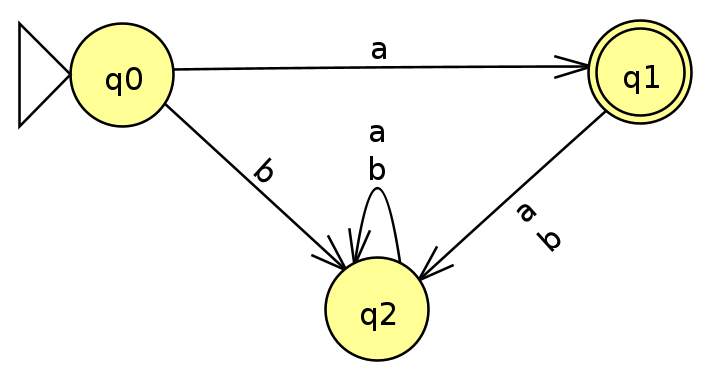
\includegraphics[scale=0.30]{images/automata.png}
\label{}
\end{figure}
\end{enumerate}

\begin{equation}
	M = (\{q_0, q_1, q_2\}, \{a, b\}, \delta, q_0, \{q_2\})
\end{equation}

\begin{table}[]
\centering
\begin{tabular}{c|c|ccc}
$\delta$(q, $\sigma$) & $a$    & $b$    &  &  \\ \cline{1-3}
$q_0$   & $q_1$ & $q_2$&  &  \\ \cline{1-3}
$q_1$   & $q_2$ & $q_2$ &  &  \\ \cline{1-3}
$q_2$    & $q_2$ & $q_2$ &  & 
\end{tabular}
\end{table}

\newpage

\begin{enumerate}
\setcounter{enumi}{1}
\item Test the automaton that you have created by introducing 6 chains.
\end{enumerate}

\begin{figure}[]
\centering
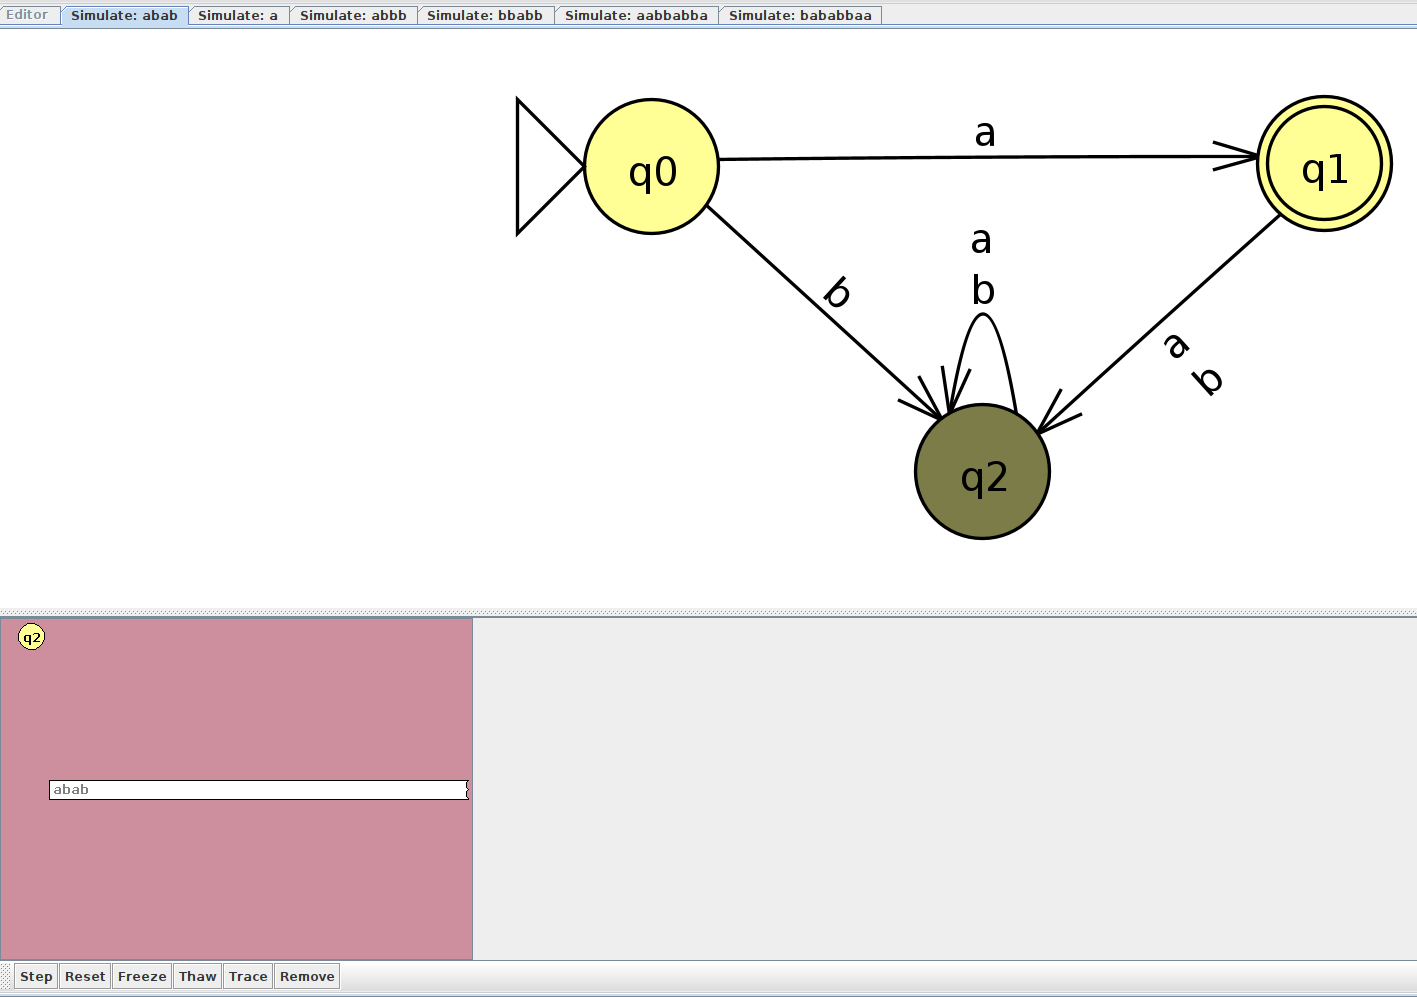
\includegraphics[scale=0.2]{images/Cadena1.png}
\label{}
\\
\centering{\textit{Prueba de la cadena "abab"}}
\end{figure}

\begin{figure}[]
\centering
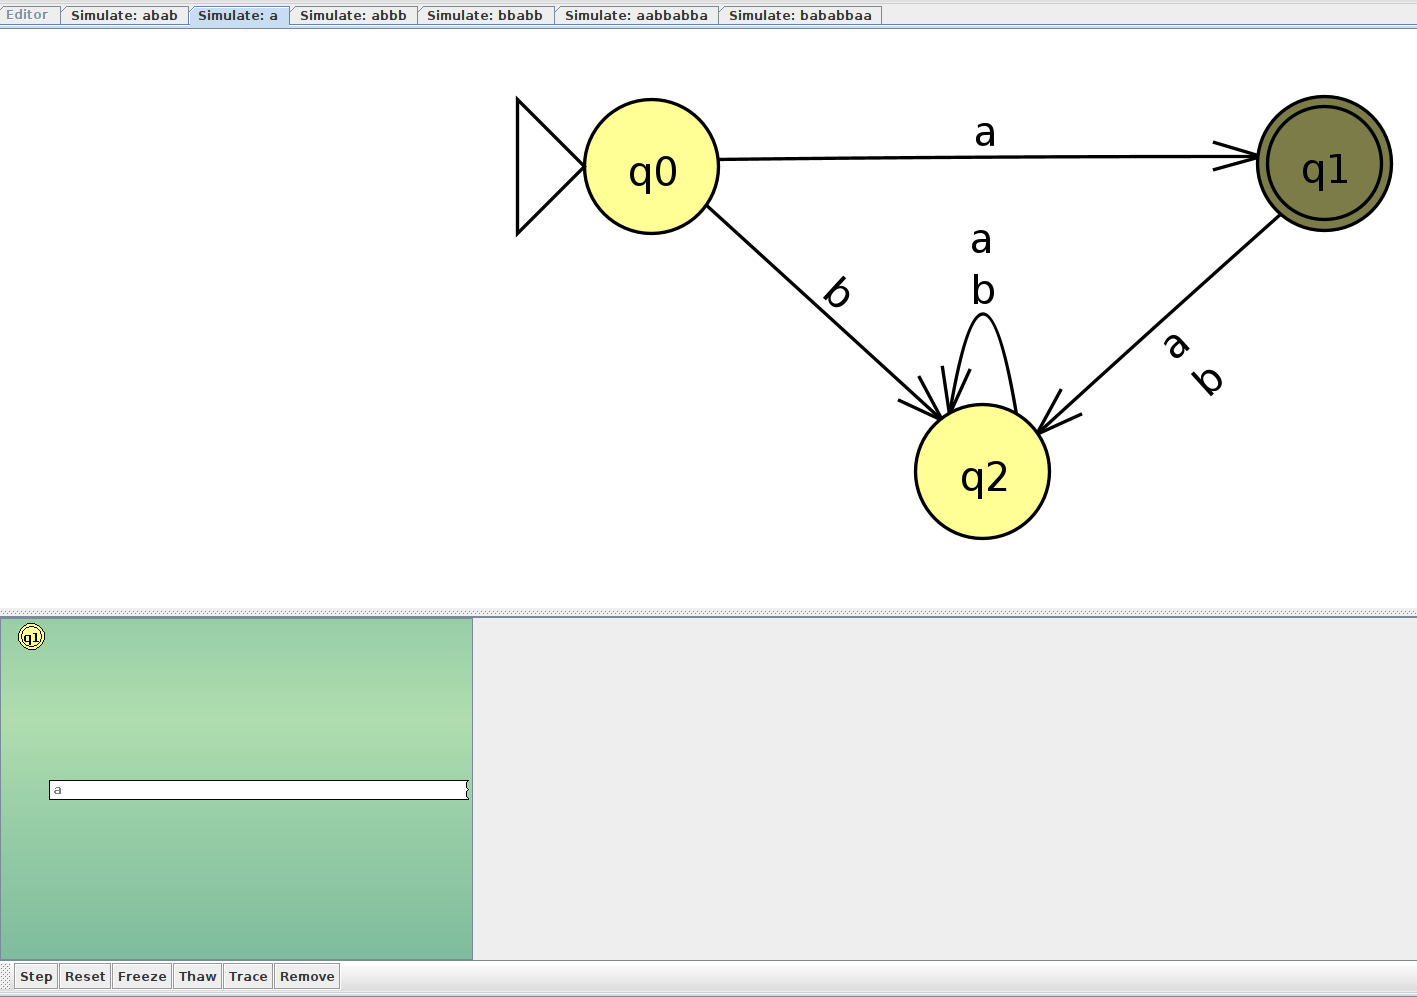
\includegraphics[scale=0.2]{images/Cadena2.png}
\label{}
\\
\centering{\textit{Prueba de la cadena "a"}}
\end{figure}

\begin{figure}[]
\centering
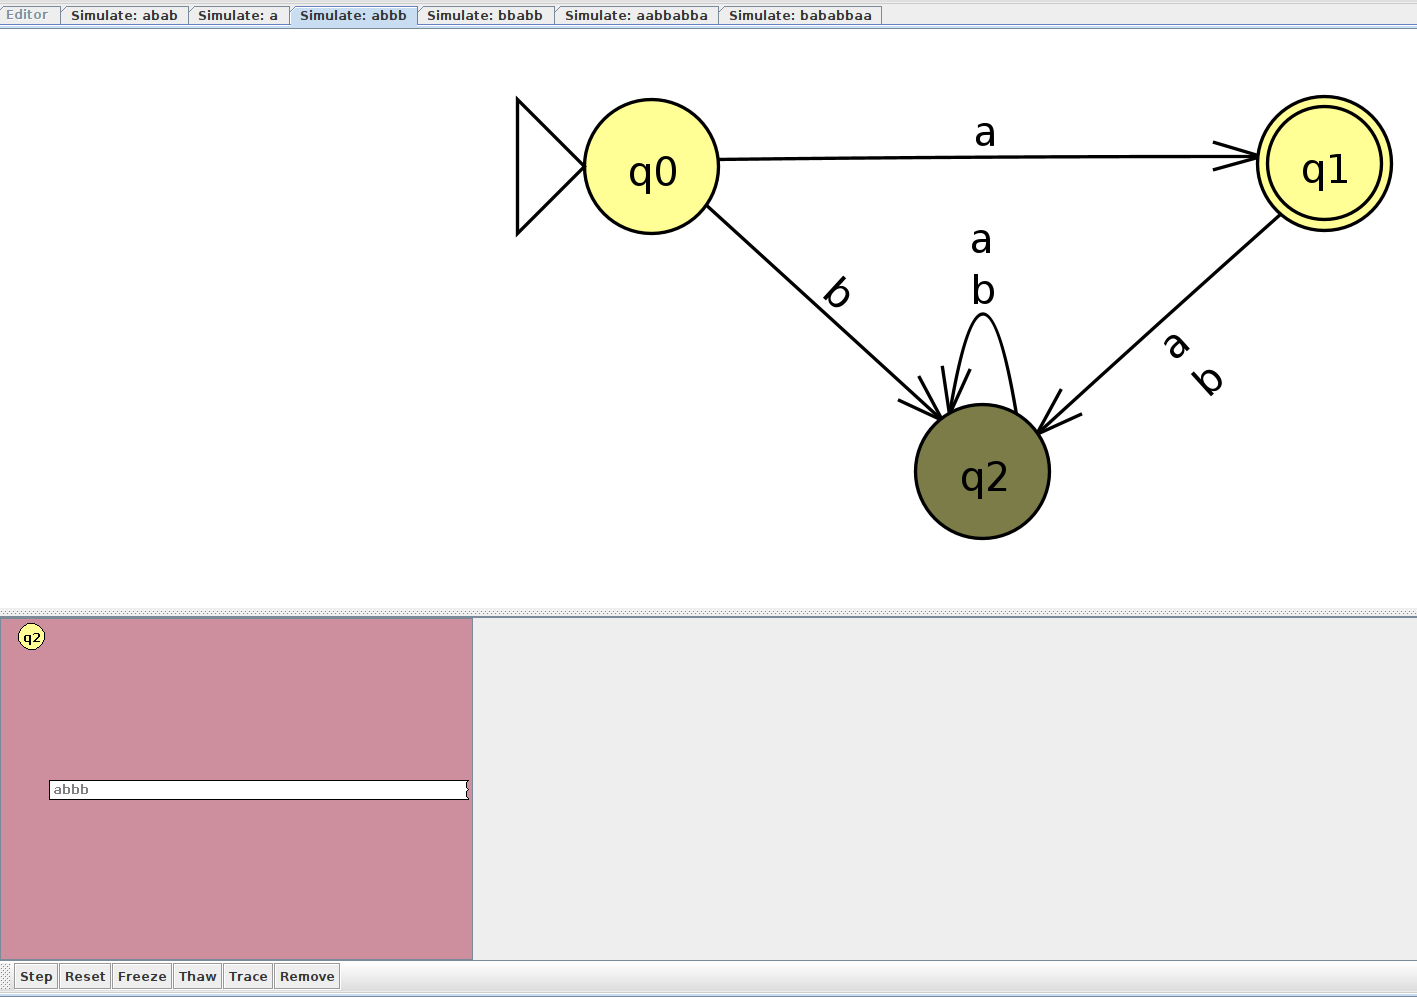
\includegraphics[scale=0.2]{images/Cadena3.png}
\label{}
\\
\centering{\textit{Prueba de la cadena "abbb"}}
\end{figure}

\begin{figure}[]
\centering
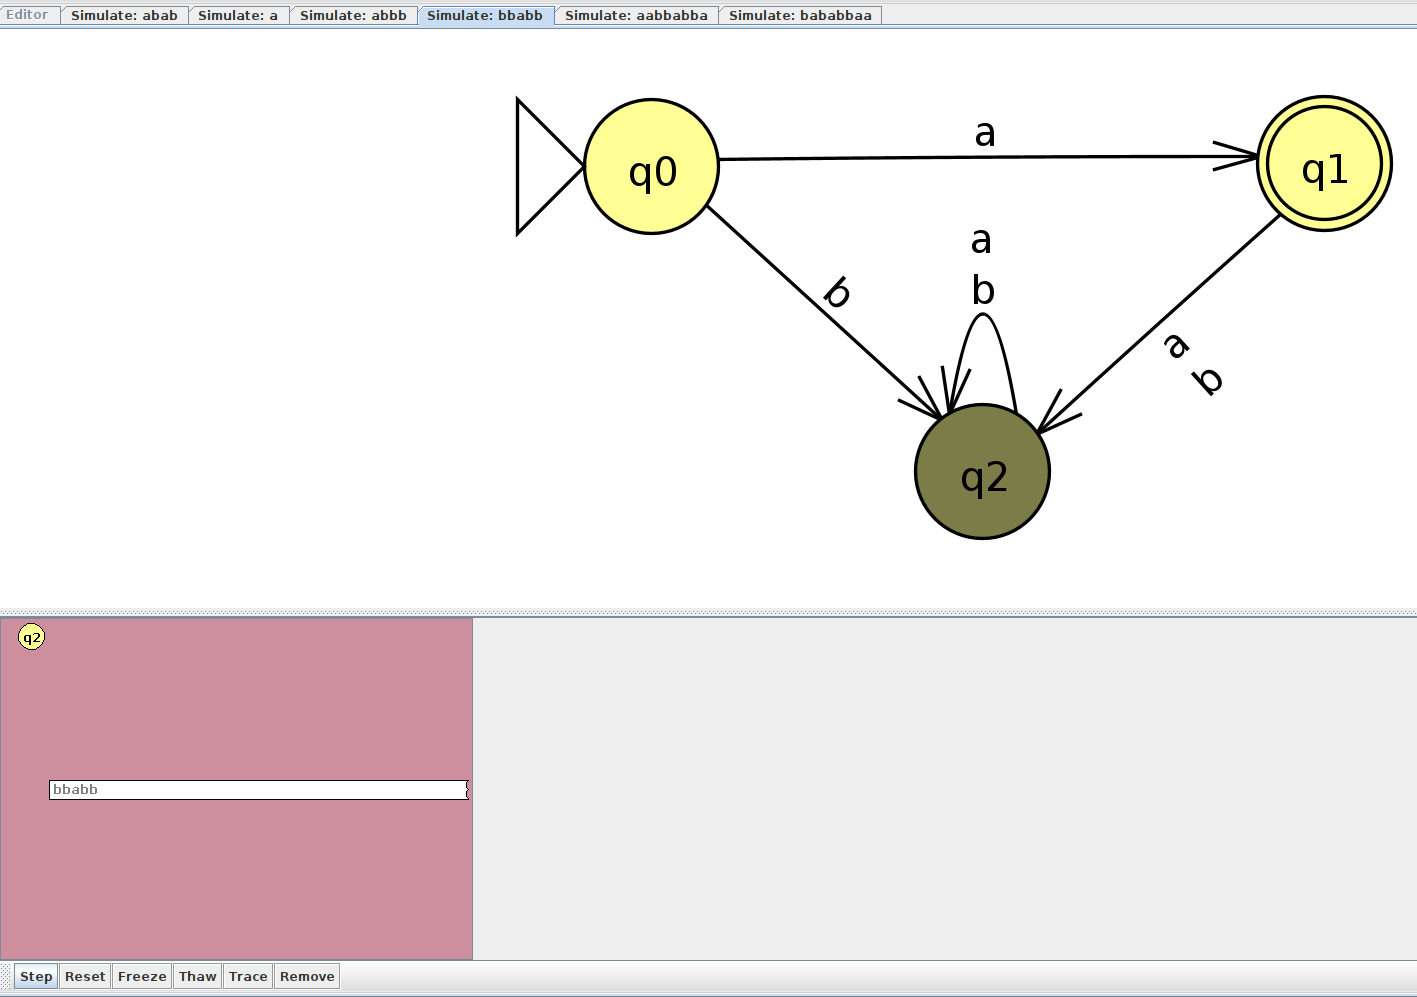
\includegraphics[scale=0.2]{images/Cadena4.png}
\label{}
\\
\centering{\textit{Prueba de la cadena "bbabb"}}
\end{figure}

\begin{figure}[]
\centering
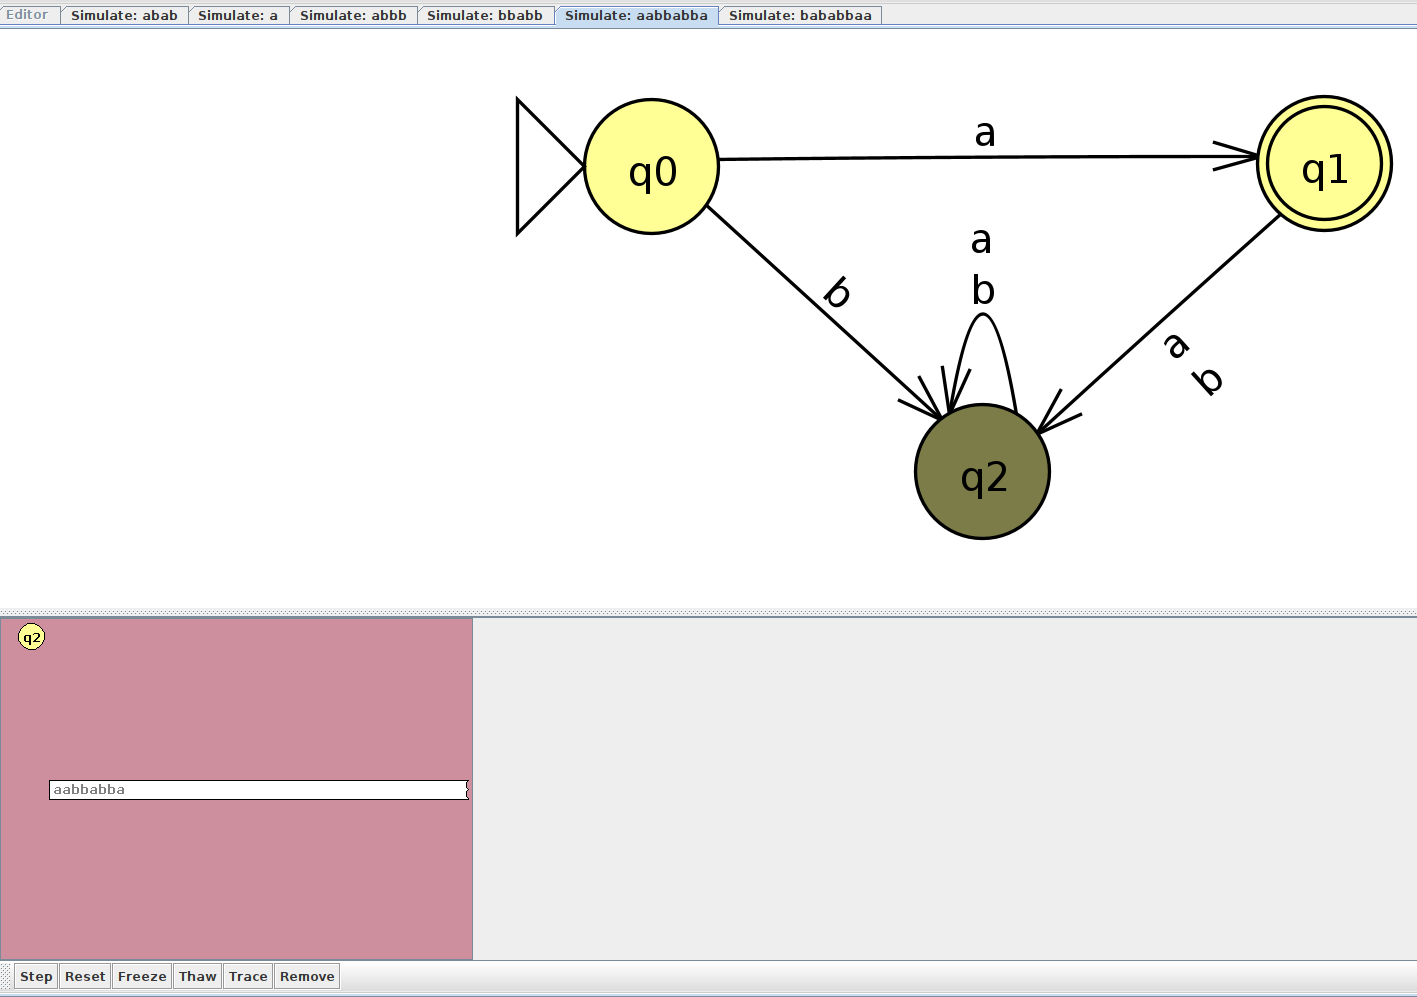
\includegraphics[scale=0.2]{images/Cadena5.png}
\label{}
\\
\centering{\textit{Prueba de la cadena "aabbabba"}}
\end{figure}

\begin{figure}[]
\centering
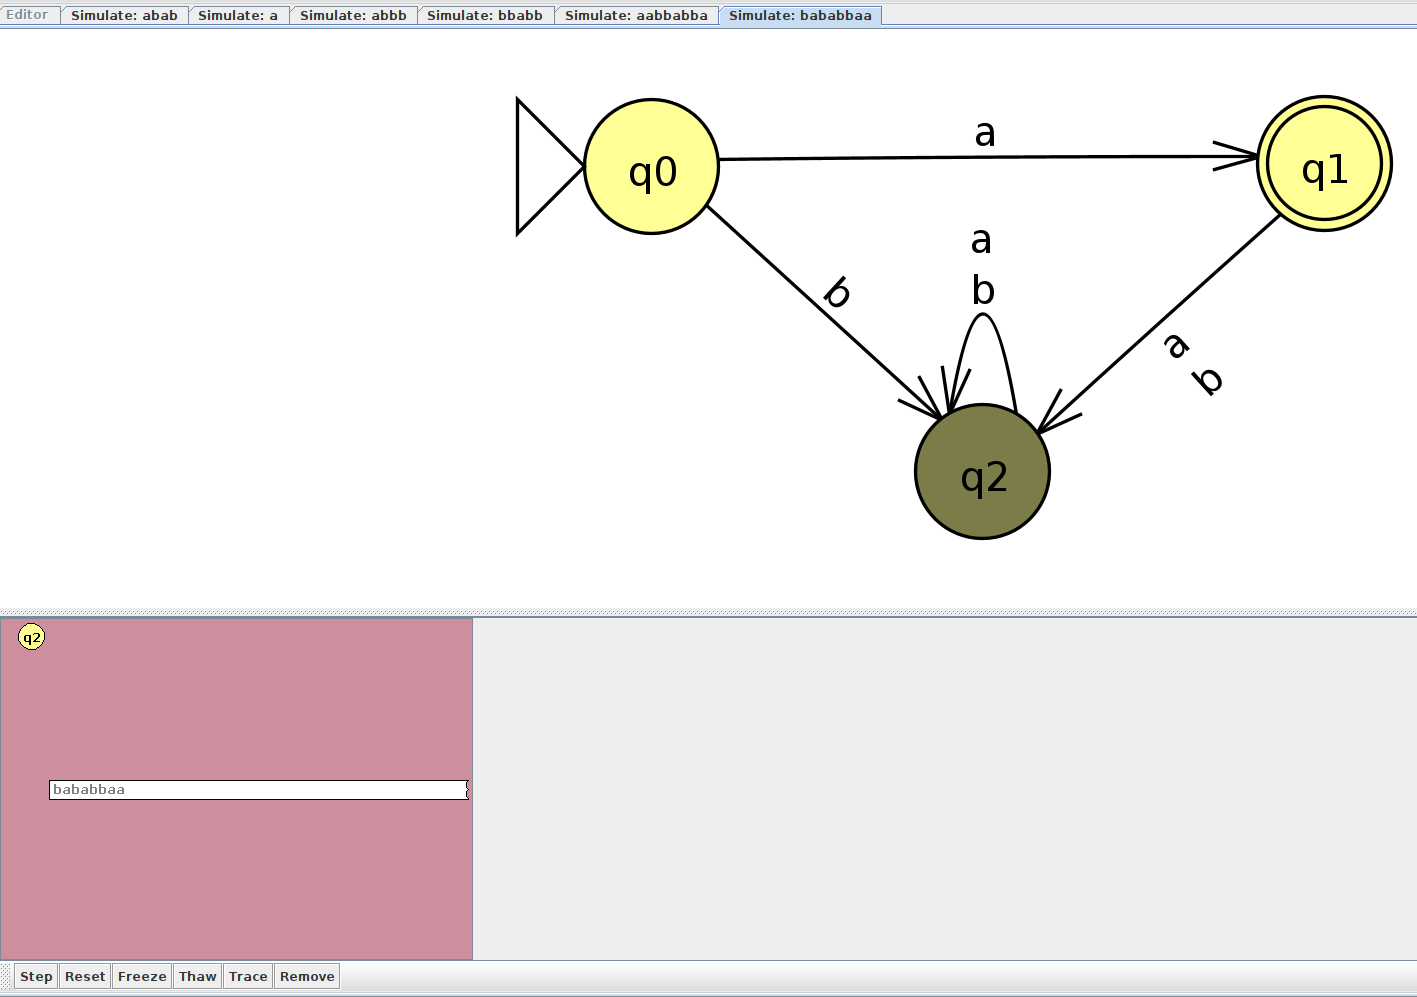
\includegraphics[scale=0.2]{images/Cadena6.png}
\label{}
\\
\centering{\textit{Prueba de la cadena "bababbaa"}}
\end{figure}

\newpage
\section*{Ejercicio 2}
Finite automaton in Octave:

\begin{enumerate}
\item Open the Octave finiteautomata.m script and test it with the given
example (see script help) in the GitHub repository.

Prueba con octave usando el script:

\begin{figure}[htp]
\centering
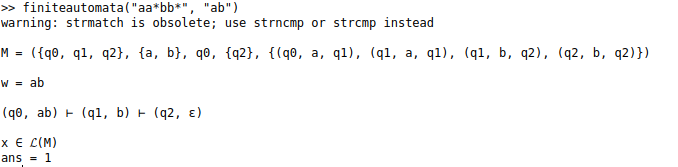
\includegraphics[scale=0.65]{images/2a.png}
\end{figure}

\end{enumerate}

\begin{enumerate}
\setcounter{enumi}{1}
\item Specify in finiteautomata.json the automaton created in Activity 1
and test it with the script!

Prueba con Octave utizando mi propio autómata en el script:

\begin{figure}[htp]
\centering
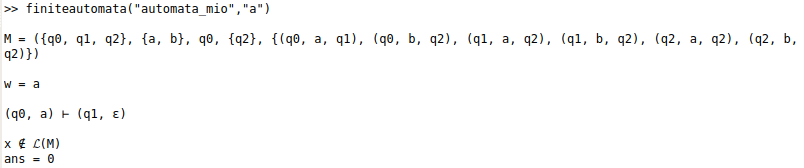
\includegraphics[scale=0.65]{images/2b.png}
\end{figure}

\end{enumerate}

\end{document}

